\documentclass[conference]{IEEEtran}
\IEEEoverridecommandlockouts
% The preceding line is only needed to identify funding in the first footnote. If that is unneeded, please comment it out.
\usepackage{cite}
\usepackage{amsmath,amssymb,amsfonts}
\usepackage{algorithmic}
\usepackage{graphicx}
\usepackage{textcomp}
\usepackage{xcolor}
\usepackage[portuguese]{babel}

\def\BibTeX{{\rm B\kern-.05em{\sc i\kern-.025em b}\kern-.08em
    T\kern-.1667em\lower.7ex\hbox{E}\kern-.125emX}}
\begin{document}

% Keywords command
\providecommand{\keywords}[1]
{
  \small	
  \textbf{\textit{Palavras-chave---}} #1
}

\title{\textit{Análise Comparativa de Algoritmos de Roteamento para o Problema do Caminho Mais Curto em Redes de Computadores}}

\author{\IEEEauthorblockN{1\textsuperscript{st} Daniel S. Silva}
\IEEEauthorblockA{\textit{Instituto de Computação} \\
\textit{Universidade Federal do Rio de Janeiro (UFRJ)}\\
Rio de Janeiro, Brasil \\
\textit{danielss@dcc.ufrj.br}}
}

\maketitle

\begin{abstract}
Este artigo apresenta uma análise comparativa entre três algoritmos de roteamento - PLisita, \textbf{Simulated Annealing (SA)} e \textbf{Simulated Annealing com a hibridização de Algoritmo Genético (Simulated AnnealingGA)} - para solucionar o problema do caminho mais curto (\textit{SPP}) em redes de computadores. O estudo foi conduzido em um grafo composto por 144 nós distribuídos aleatoriamente. O objetivo foi alcançar dois roteadores específicos, o 119 e o 70, através da execução do programa \textit{SinalGo} em 30 iterações para cada algoritmo.

Os valores de \textit{EstimatedRTT}, \textit{DevRTT} e \textit{Timeout Interval} foram calculados com base nos dados coletados, utilizando os coeficientes alfa (0,125) e beta (0,25). Os resultados revelaram que o algoritmo de \textbf{Simulated Annealing} demonstrou um desempenho superior em ambas as situações propostas. Especificamente, ao considerar os valores médios do \textit{Timeout Interval}, o \textbf{Simulated Annealing} mostrou-se mais eficiente em comparação com os demais algoritmos analisados.

Os dados coletados indicaram consistentemente que o \textit{Timeout Interval} obtido pelo \textbf{Simulated Annealing} foi significativamente menor do que os valores encontrados nos outros algoritmos avaliados. Esses achados enfatizam a robustez e a adequação do \textbf{Simulated Annealing} para possíveis implementações em Sistemas Autônomos (AS) em redes de computadores reais.
\end{abstract}

\keywords{Otimização, algoritmos evolutivos, problema do caminho mais curto, rede de computadores}

\section{Introdução}
O roteamento de pacotes é um elemento essencial nas redes de computadores, sendo o processo pelo qual os dispositivos direcionam e entregam informações na Internet. Na prática, cada dispositivo, ao receber um pacote, utiliza algoritmos de roteamento para determinar o próximo destino apropriado, seguindo um modelo conhecido como hop-by-hop. A eficácia desses algoritmos é crucial para encontrar caminhos adequados para a transmissão eficiente dos dados.

Para isso, são utilizadas tabelas de roteamento e protocolos específicos. Essas tabelas contêm informações essenciais, como os endereços dos membros da rede, e os protocolos definem as rotas ideais para o envio dos pacotes. Além disso, na Internet, a estrutura hierárquica de Sistemas Autônomos (ASs) desempenha um papel fundamental, permitindo a divisão de redes e a execução de protocolos de roteamento específicos para resolver questões de escala e autoridade administrativa.

Neste contexto, diferentes protocolos como RIP (\textit{Routing Information Protocol}), OSPF (\textit{Open Shortest Path First}) e BGP (\textit{Border Gateway Protocol}) são fundamentais para o roteamento interno e externo entre Sistemas Autônomos. Eles desempenham papéis específicos no funcionamento da Internet, influenciando diretamente a eficiência e a confiabilidade do processo de roteamento \cite{KuroseRoss2010}.

Este estudo visa analisar e comparar o desempenho de três algoritmos de roteamento - \textbf{PLisita}, \textbf{Simulated Annealing (SA)} e \textbf{Simulated Annealing com hibridização de Algoritmo Genético (Simulated AnnealingGA)} - na resolução do problema do caminho mais curto (\textit{SPP}) em redes de computadores, baseando-se no trabalho desenvolvido por Fonseca et al. (2022) no artigo intitulado "Active GA Accelerated by Simulated Annealing to Solve SPP in Packet Networks" \cite{OL2ARouter}.

\section{Fundamentos Teóricos}

O algoritmo de roteamento e sua aplicação pertencem à camada de rede dentro da arquitetura de redes de computadores. A camada de rede é responsável pela determinação de caminhos e roteamento dos pacotes de um remetente para um destinatário na rede.

Segundo Kurose e Ross (2010), o roteamento é um processo crítico na camada de rede. Quando um pacote chega a um roteador, este busca em uma tabela de repasse a interface de enlace para onde o pacote deve ser encaminhado. Os algoritmos de roteamento executados nos roteadores são fundamentais para troca e cálculo das informações utilizadas na configuração dessas tabelas de repasse.

O propósito central de um algoritmo de roteamento é encontrar um caminho eficiente entre um roteador de origem e um roteador de destino. Normalmente, um caminho eficiente é definido como aquele com o "menor custo". No entanto, preocupações do mundo real, como políticas de rede e questões de autoridade administrativa, podem complicar esses algoritmos.

Esses algoritmos podem ser classificados de várias maneiras. Algoritmos de estado de enlace, por exemplo, consideram a conectividade e o custo de cada enlace na rede, enquanto algoritmos de vetor de distâncias mantêm um vetor de estimativas de custo de um nó para todos os outros nós da rede. Além disso, eles podem ser estáticos ou dinâmicos, sensíveis ou insensíveis à carga.

Os algoritmos de roteamento desempenham papéis fundamentais na Internet, influenciando diretamente a eficiência e a confiabilidade do processo de roteamento \cite{KuroseRoss2010}.

\section{Experimentação e Resultados}

Os experimentos foram conduzidos para analisar o desempenho dos algoritmos de roteamento - \textbf{PLisita}, \textbf{Simulated Annealing (SA)} e \textbf{Simulated Annealing com hibridização de Algoritmo Genético (Simulated AnnealingGA)} - na resolução do Problema do Caminho Mais Curto (\textit{SPP}) em redes de computadores. Foram coletados dados de \textit{SampleRTT}, \textit{EstimatedRTT}, \textit{DevRTT} e \textit{Timeout Interval} para cada algoritmo, com o objetivo de alcançar os roteadores 119 e 70 em um grafo de 144 nós, distribuídos aleatoriamente, utilizando o programa \textit{SinalGo}.

\subsection{Métrica Utilizada}
A métrica-chave para avaliar o desempenho dos algoritmos foi o \textit{Timeout Interval}, representando o intervalo de tempo limite para uma resposta. Isso é crucial para determinar a eficiência e a confiabilidade de cada algoritmo na resolução do problema do caminho mais curto (\textit{SPP}) em redes de computadores. Quanto menor o \textit{Timeout Interval}, maior é a eficiência do algoritmo de roteamento na transmissão dos pacotes.

\subsection{Roteador 119}

\begin{itemize}
    \item \textbf{PLisita}: \textit{Timeout Interval} médio: 3,943969163
    \item \textbf{Simulated Annealing}: \textit{Timeout Interval} médio: 2,862471221
    \item \textbf{Simulated AnnealingGA}: \textit{Timeout Interval} médio: 5,064786169
\end{itemize}

\begin{figure}[h]
    \centering
    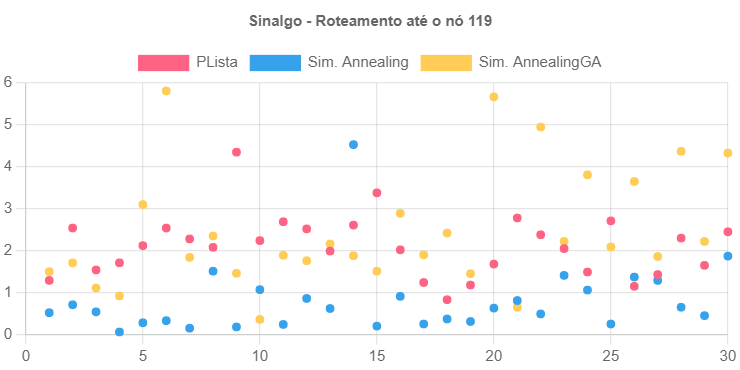
\includegraphics[width=0.5\textwidth]{chart_timeout_interval_119}
    \caption{Gráfico da simulação com objetivo no roteador 119 (Timeout Interval x Execução).}
    \label{fig:exemplo}
\end{figure}

Ao considerar o \textit{Timeout Interval} médio, o algoritmo de \textbf{Simulated Annealing} demonstrou uma eficiência superior, com um valor médio de \textit{Timeout Interval} de aproximadamente 2,86, comparado a aproximadamente 3,94 e 5,06 dos algoritmos \textbf{PLisita} e \textbf{Simulated AnnealingGA}, respectivamente. Isso sugere uma capacidade mais eficaz do algoritmo \textbf{Simulated Annealing} para alcançar o roteador 119 em tempo menor, tornando-o mais adequado para essa tarefa específica.

\subsection{Roteador 70}

\begin{itemize}
    \item \textbf{PLisita}: \textit{Timeout Interval} médio: 6,886985561
    \item \textbf{Simulated Annealing}: \textit{Timeout Interval} médio: 4,562312878
    \item \textbf{Simulated AnnealingGA}: \textit{Timeout Interval} médio: 11,35125801
\end{itemize}

\begin{figure}[h]
    \centering
    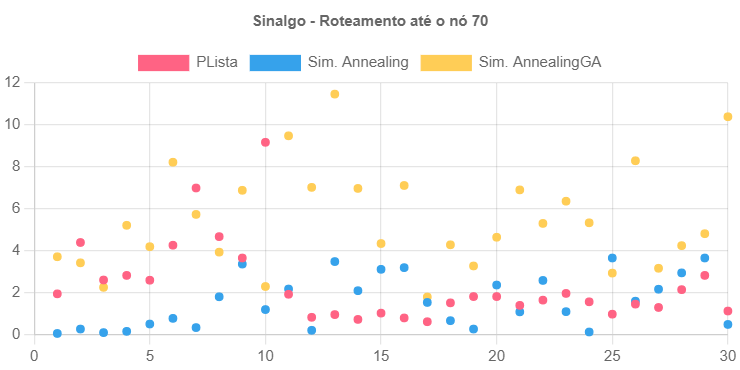
\includegraphics[width=0.5\textwidth]{chart_timeout_interval_70}
    \caption{Gráfico da simulação com objetivo no roteador 70 (Timeout Interval x Execução).}
    \label{fig:exemplo}
\end{figure}

Da mesma forma, ao analisar o \textit{Timeout Interval} médio para alcançar o roteador 70, observa-se que o algoritmo \textbf{Simulated Annealing} obteve um valor médio de \textit{Timeout Interval} de cerca de 4,56, enquanto \textbf{PLisita} e \textbf{Simulated AnnealingGA} tiveram valores médios de aproximadamente 6,89 e 11,35, respectivamente. Isso reforça a superioridade do algoritmo \textbf{Simulated Annealing} na eficiência de roteamento para o roteador 70, indicando sua vantagem em alcançar esse destino em um tempo menor.

Portanto, com base nos resultados do \textit{Timeout Interval} médio, o algoritmo de \textbf{Simulated Annealing} se destaca como a escolha preferencial para alcançar tanto o roteador 119 quanto o roteador 70 em comparação com os outros algoritmos analisados. Esses resultados sugerem que o \textbf{Simulated Annealing} pode ser mais adequado para implementações práticas em Sistemas Autônomos (AS) dentro de redes de computadores reais, fornecendo eficiência no roteamento de pacotes com menor tempo de espera.

\section{Conclusão}

Com base nos resultados obtidos a partir dos experimentos realizados, fica claro que o algoritmo de \textbf{Simulated Annealing} se destaca como uma solução altamente eficiente para resolver o problema do caminho mais curto em roteamento de redes de computadores. Ao analisar os valores médios de \textit{Timeout Interval} nas duas situações propostas - alcançar os roteadores 119 e 70 - torna-se evidente que o \textbf{Simulated Annealing} supera consistentemente os demais algoritmos avaliados.

Estes resultados refletem a capacidade excepcional do \textbf{Simulated Annealing} em oferecer um desempenho superior, destacando-se pela sua rápida convergência e eficiência em comparação com outras abordagens. Essa superioridade reforça a viabilidade e a robustez deste algoritmo para aplicação prática em redes de computadores reais, com potencial impacto positivo em Sistemas Autônomos.

\begin{thebibliography}{00}
\bibitem{KuroseRoss2010}
Kurose, J. F., \& Ross, K. W. (2010). \textit{Redes de Computadores e a Internet: uma abordagem top-down} (5ª ed.). São Paulo: Addison Wesley.

\bibitem{OL2ARouter}
Fonseca, D.S., Wanner, E.F., Marcelino, C.G., Silva, G.P., Jimenez-Fernandez, S., Salcedo-Sanz, S. (2022). Active GA Accelerated by Simulated Annealing to Solve SPP in Packet Networks. In: Pereira, A.I., Košir, A., Fernandes, F.P., Pacheco, M.F., Teixeira, J.P., Lopes, R.P. (eds) Optimization, Learning Algorithms and Applications. OL2A 2022. Communications in Computer and Information Science, vol 1754. Springer, Cham. https://doi.org/10.1007/978-3-031-23236-7\_24
\end{thebibliography} 
\end{document}
